% $Header: /u/gcmpack/manual/s_overview/text/manual.tex,v 1.18 2004/03/23 15:29:39 afe Exp $
% $Name:  $

%tci%\documentclass[12pt]{book}
%tci%\usepackage{amsmath}
%tci%\usepackage{html}
%tci%\usepackage{epsfig}
%tci%\usepackage{graphics,subfigure}
%tci%\usepackage{array}
%tci%\usepackage{multirow}
%tci%\usepackage{fancyhdr}
%tci%\usepackage{psfrag}

%tci%%TCIDATA{OutputFilter=Latex.dll}
%tci%%TCIDATA{LastRevised=Thursday, October 04, 2001 14:41:22}
%tci%%TCIDATA{<META NAME="GraphicsSave" CONTENT="32">}
%tci%%TCIDATA{Language=American English}

%tci%\fancyhead{}
%tci%\fancyhead[LO]{\slshape \rightmark}
%tci%\fancyhead[RE]{\slshape \leftmark}
%tci%\fancyhead[RO,LE]{\thepage}
%tci%\fancyfoot[CO,CE]{\today}
%tci%\fancyfoot[RO,LE]{ }
%tci%\renewcommand{\headrulewidth}{0.4pt}
%tci%\renewcommand{\footrulewidth}{0.4pt}
%tci%\setcounter{secnumdepth}{3}
%tci%\input{tcilatex}

%tci%\begin{document}

%tci%\tableofcontents


% Section: Overview

% $Header: /u/gcmpack/manual/s_overview/text/manual.tex,v 1.18 2004/03/23 15:29:39 afe Exp $
% $Name:  $

This document provides the reader with the information necessary to
carry out numerical experiments using MITgcm. It gives a comprehensive
description of the continuous equations on which the model is based, the
numerical algorithms the model employs and a description of the associated
program code. Along with the hydrodynamical kernel, physical and
biogeochemical parameterizations of key atmospheric and oceanic processes
are available. A number of examples illustrating the use of the model in
both process and general circulation studies of the atmosphere and ocean are
also presented.

\section{Introduction}
\begin{rawhtml}
<!-- CMIREDIR:innovations -->
\end{rawhtml}


MITgcm has a number of novel aspects:

\begin{itemize}
\item it can be used to study both atmospheric and oceanic phenomena; one
hydrodynamical kernel is used to drive forward both atmospheric and oceanic
models - see fig \ref{fig:onemodel}

%% CNHbegin
\begin{figure}
\begin{center}
 \includegraphics*[width=.9\textwidth]{part1/onemodel.eps}
\end{center}
\caption{MITgcm has a single dynamical kernel that can drive forward
either oceanic or atmospheric simulations.}
\label{fig:onemodel}
\end{figure}

%% CNHend

\item it has a non-hydrostatic capability and so can be used to study both
small-scale and large scale processes - see fig \ref{fig:all-scales}

%% CNHbegin
\begin{figure}
 \rotatebox{90}{
 \rotatebox{180}{
  \resizebox{3.2in}{6.5in}{
   \includegraphics*[0.5in,0.5in][6.5in,12.5in]{part1/scales.eps}
  }
 }
 }
\caption{MITgcm has non-hydrostatic capabilities, allowing
the model to address a wide range of phenomenon - from convection
on the left, all the way through to global circulation patterns on the 
right.
}
\label{fig:all-scales}
\end{figure}

%% CNHend

\item finite volume techniques are employed yielding an intuitive
discretization and support for the treatment of irregular geometries using
orthogonal curvilinear grids and shaved cells - see fig \ref{fig:finite-volumes}

%% CNHbegin
\begin{figure}
  \resizebox{6.2in}{4.5in}{
   \includegraphics*[3.0in,0.5in][9.5in,7.15in]{part1/fvol.eps}
  }
\caption{Finite volume techniques (bottom panel) are user, permitting
a treatment of topography that rivals $\sigma$ (terrain following)
coordinates.}
\label{fig:finite-volumes}
\end{figure}

%% CNHend

\item tangent linear and adjoint counterparts are automatically maintained
along with the forward model, permitting sensitivity and optimization
studies.

\item the model is developed to perform efficiently on a wide variety of
computational platforms.
\end{itemize}

Key publications reporting on and charting the development of the model are
\cite{hill:95,marshall:97a,marshall:97b,adcroft:97,marshall:98,adcroft:99,hill:99,maro-eta:99}:

\begin{verbatim}
Hill, C. and J. Marshall, (1995)
Application of a Parallel Navier-Stokes Model to Ocean Circulation in 
Parallel Computational Fluid Dynamics
In Proceedings of Parallel Computational Fluid Dynamics: Implementations 
and Results Using Parallel Computers, 545-552.
Elsevier Science B.V.: New York

Marshall, J., C. Hill, L. Perelman, and A. Adcroft, (1997)
Hydrostatic, quasi-hydrostatic, and nonhydrostatic ocean modeling
J. Geophysical Res., 102(C3), 5733-5752.

Marshall, J., A. Adcroft, C. Hill, L. Perelman, and C. Heisey, (1997)
A finite-volume, incompressible Navier Stokes model for studies of the ocean
on parallel computers,
J. Geophysical Res., 102(C3), 5753-5766.

Adcroft, A.J., Hill, C.N. and J. Marshall, (1997)
Representation of topography by shaved cells in a height coordinate ocean
model
Mon Wea Rev, vol 125, 2293-2315

Marshall, J., Jones, H. and C. Hill, (1998)
Efficient ocean modeling using non-hydrostatic algorithms
Journal of Marine Systems, 18, 115-134

Adcroft, A., Hill C. and J. Marshall: (1999)
A new treatment of the Coriolis terms in C-grid models at both high and low
resolutions,
Mon. Wea. Rev. Vol 127, pages 1928-1936

Hill, C, Adcroft,A., Jamous,D., and J. Marshall, (1999)
A Strategy for Terascale Climate Modeling.
In Proceedings of the Eighth ECMWF Workshop on the Use of Parallel Processors
in Meteorology, pages 406-425
World Scientific Publishing Co: UK

Marotzke, J, Giering,R., Zhang, K.Q., Stammer,D., Hill,C., and T.Lee, (1999)
Construction of the adjoint MIT ocean general circulation model and 
application to Atlantic heat transport variability
J. Geophysical Res., 104(C12), 29,529-29,547.

\end{verbatim}

We begin by briefly showing some of the results of the model in action to
give a feel for the wide range of problems that can be addressed using it.

% $Header: /u/gcmpack/manual/s_overview/text/manual.tex,v 1.18 2004/03/23 15:29:39 afe Exp $
% $Name:  $

\section{Illustrations of the model in action}

The MITgcm has been designed and used to model a wide range of phenomena,
from convection on the scale of meters in the ocean to the global pattern of
atmospheric winds - see figure \ref{fig:all-scales}. To give a flavor of the
kinds of problems the model has been used to study, we briefly describe some
of them here. A more detailed description of the underlying formulation,
numerical algorithm and implementation that lie behind these calculations is
given later. Indeed many of the illustrative examples shown below can be
easily reproduced: simply download the model (the minimum you need is a PC
running Linux, together with a FORTRAN\ 77 compiler) and follow the examples
described in detail in the documentation.

\subsection{Global atmosphere: `Held-Suarez' benchmark}
\begin{rawhtml}
<!-- CMIREDIR:atmospheric_example -->
\end{rawhtml}



A novel feature of MITgcm is its ability to simulate, using one basic algorithm, 
both atmospheric and oceanographic flows at both small and large scales.

Figure \ref{fig:eddy_cs} shows an instantaneous plot of the 500$mb$
temperature field obtained using the atmospheric isomorph of MITgcm run at
2.8$^{\circ }$ resolution on the cubed sphere. We see cold air over the pole
(blue) and warm air along an equatorial band (red). Fully developed
baroclinic eddies spawned in the northern hemisphere storm track are
evident. There are no mountains or land-sea contrast in this calculation,
but you can easily put them in. The model is driven by relaxation to a
radiative-convective equilibrium profile, following the description set out
in Held and Suarez; 1994 designed to test atmospheric hydrodynamical cores -
there are no mountains or land-sea contrast.

%% CNHbegin
\begin{figure}
  \resizebox{4.5in}{4.5in}{
   \includegraphics*[1.5in,1.5in][8.5in,8.5in]{part1/eddy_on_cubic_globe.eps}
 }
\caption{}
\label{fig:eddy_cs}
\end{figure}

%% CNHend

As described in Adcroft (2001), a `cubed sphere' is used to discretize the
globe permitting a uniform griding and obviated the need to Fourier filter.
The `vector-invariant' form of MITgcm supports any orthogonal curvilinear
grid, of which the cubed sphere is just one of many choices.

Figure \ref{fig:hs_zave_u} shows the 5-year mean, zonally averaged zonal
wind from a 20-level configuration of
the model. It compares favorable with more conventional spatial
discretization approaches. The two plots show the field calculated using the
cube-sphere grid and the flow calculated using a regular, spherical polar
latitude-longitude grid. Both grids are supported within the model.

%% CNHbegin
\begin{figure}
 \begin{center}
   \includegraphics*[width=.9\textwidth]{part1/u_cube.ps}
   \includegraphics*[width=.9\textwidth]{part1/u_latlon.ps}
 \end{center}
\caption{Five year mean, zonally averaged zonal flow for latitude-longitude
simulation (left) and cube-sphere simulation (right) using Held-Suarez
forcing. Both solutions compare favorably with reference solutions.}
\label{fig:hs_zave_u}
\end{figure}

%% CNHend

\subsection{Ocean gyres}
\begin{rawhtml}
<!-- CMIREDIR:oceanic_example -->
\end{rawhtml}
\begin{rawhtml}
<!-- CMIREDIR:ocean_gyres -->
\end{rawhtml}

Baroclinic instability is a ubiquitous process in the ocean, as well as the
atmosphere. Ocean eddies play an important role in modifying the
hydrographic structure and current systems of the oceans. Coarse resolution
models of the oceans cannot resolve the eddy field and yield rather broad,
diffusive patterns of ocean currents. But if the resolution of our models is
increased until the baroclinic instability process is resolved, numerical
solutions of a different and much more realistic kind, can be obtained.

Figure \ref{fig:ocean-gyres} shows the surface temperature and velocity 
field obtained from MITgcm run at $\frac{1}{6}^{\circ }$ horizontal 
resolution on a $lat-lon$
grid in which the pole has been rotated by 90$^{\circ }$ on to the equator
(to avoid the converging of meridian in northern latitudes). 21 vertical
levels are used in the vertical with a `lopped cell' representation of
topography. The development and propagation of anomalously warm and cold
eddies can be clearly seen in the Gulf Stream region. The transport of
warm water northward by the mean flow of the Gulf Stream is also clearly
visible.

%% CNHbegin
\begin{figure}
 \begin{center}
  \includegraphics*[angle=-90,width=.9\textwidth]{part1/atl6.eps}
 \end{center}
\caption{Instantaneous temperature map from a $\frac{1}{6}^{\circ }$
simulation of the North Atlantic. The figure
shows the temperature in the second layer (37.5m
deep).}
\label{fig:ocean-gyres}
\end{figure}

%% CNHend


\subsection{Global ocean circulation}
\begin{rawhtml}
<!-- CMIREDIR:global_ocean_circulation -->
\end{rawhtml}

Figure \ref{fig:large-scale-circ} (top) shows the pattern of ocean currents at 
the surface of a 4$^{\circ }$
global ocean model run with 15 vertical levels. Lopped cells are used to
represent topography on a regular $lat-lon$ grid extending from 70$^{\circ
}N $ to 70$^{\circ }S$. The model is driven using monthly-mean winds with
mixed boundary conditions on temperature and salinity at the surface. The
transfer properties of ocean eddies, convection and mixing is parameterized
in this model.

Figure \ref{fig:large-scale-circ} (bottom) shows the meridional overturning 
circulation of the global ocean in Sverdrups.

%%CNHbegin
\begin{rawhtml}MITGCM_INSERT_FIGURE_BEGIN large-scale-circ\end{rawhtml}
\begin{figure}
\begin{center}
 \includegraphics*[width=.8\textwidth,bb=65 70 510 390]{s_overview/figs/isovec_atmoce_new.ps}
 \includegraphics*[width=.8\textwidth]{s_overview/figs/moc.eps}
\end{center}
\caption{Pattern of surface ocean currents (top) and meridional
overturning stream function (in Sverdrups) from a global
integration of the model at $4^{\circ}$ horizontal resolution and with
15 vertical levels.}
\label{fig:large-scale-circ}
\end{figure}
\begin{rawhtml}MITGCM_INSERT_FIGURE_END\end{rawhtml}

%%CNHend

\subsection{Convection and mixing over topography}
\begin{rawhtml}
<!-- CMIREDIR:mixing_over_topography -->
\end{rawhtml}


Dense plumes generated by localized cooling on the continental shelf of the
ocean may be influenced by rotation when the deformation radius is smaller
than the width of the cooling region. Rather than gravity plumes, the
mechanism for moving dense fluid down the shelf is then through geostrophic
eddies. The simulation shown in the figure \ref{fig:convect-and-topo}
(blue is cold dense fluid, red is
warmer, lighter fluid) employs the non-hydrostatic capability of MITgcm to
trigger convection by surface cooling. The cold, dense water falls down the
slope but is deflected along the slope by rotation. It is found that
entrainment in the vertical plane is reduced when rotational control is
strong, and replaced by lateral entrainment due to the baroclinic
instability of the along-slope current.

%%CNHbegin
\begin{figure}
  \resizebox{6.2in}{3.5in}{
   \includegraphics*[0.5in,2.5in][6.5in,8.0in]{part1/Tt4000.eps}
  }
\caption{}
\label{fig:convect-and-topo}
\end{figure}

%%CNHend

\subsection{Boundary forced internal waves}
\begin{rawhtml}
<!-- CMIREDIR:boundary_forced_internal_waves -->
\end{rawhtml}

The unique ability of MITgcm to treat non-hydrostatic dynamics in the
presence of complex geometry makes it an ideal tool to study internal wave
dynamics and mixing in oceanic canyons and ridges driven by large amplitude
barotropic tidal currents imposed through open boundary conditions.

Fig. \ref{fig:boundary-forced-wave} shows the influence of cross-slope 
topographic variations on
internal wave breaking - the cross-slope velocity is in color, the density
contoured. The internal waves are excited by application of open boundary
conditions on the left. They propagate to the sloping boundary (represented
using MITgcm's finite volume spatial discretization) where they break under
nonhydrostatic dynamics.

%%CNHbegin
\begin{figure}
  \resizebox{5.0in}{3.5in}{
   \includegraphics*[0.5in,2.5in][6.5in,8.5in]{part1/TUt8000slope.eps}
  }
\caption{}
\label{fig:boundary-forced-wave}
\end{figure}

%%CNHend

\subsection{Parameter sensitivity using the adjoint of MITgcm}
\begin{rawhtml}
<!-- CMIREDIR:parameter_sensitivity -->
\end{rawhtml}

Forward and tangent linear counterparts of MITgcm are supported using an
`automatic adjoint compiler'. These can be used in parameter sensitivity and
data assimilation studies.

As one example of application of the MITgcm adjoint, Figure \ref{fig:hf-sensitivity}
maps the gradient $\frac{\partial J}{\partial \mathcal{H}}$where $J$ is the magnitude
of the overturning stream-function shown in figure \ref{fig:large-scale-circ}
at 60$^{\circ }$N and $
\mathcal{H}(\lambda,\varphi)$ is the mean, local air-sea heat flux over
a 100 year period. We see that $J$ is
sensitive to heat fluxes over the Labrador Sea, one of the important sources
of deep water for the thermohaline circulations. This calculation also
yields sensitivities to all other model parameters.

%%CNHbegin
\begin{rawhtml}MITGCM_INSERT_FIGURE_BEGIN hf-sensitivity\end{rawhtml}
\begin{figure}
  \begin{center}
   \includegraphics*[width=\textwidth,trim=0 0 0 40]{s_overview/figs/adj_hf_ocean.eps}
  \end{center}
\caption{Sensitivity of meridional overturning strength to surface heat flux
changes. Contours show the magnitude of the response (in ${\rm Sv }\times 10^{-4}$) that a persistent
$+1{\rm W}{\rm m}^{-2}$ heat flux anomaly at a given gid point would
produce.}
\label{fig:hf-sensitivity}
\end{figure}
\begin{rawhtml}MITGCM_INSERT_FIGURE_END\end{rawhtml}

%%CNHend

\subsection{Global state estimation of the ocean}
\begin{rawhtml}
<!-- CMIREDIR:global_state_estimation -->
\end{rawhtml}


An important application of MITgcm is in state estimation of the global
ocean circulation. An appropriately defined `cost function', which measures
the departure of the model from observations (both remotely sensed and
in-situ) over an interval of time, is minimized by adjusting `control
parameters' such as air-sea fluxes, the wind field, the initial conditions
etc. Figure \ref{fig:assimilated-globes} shows the large scale planetary
circulation and a Hopf-Muller plot of Equatorial sea-surface height.
Both are obtained from assimilation bringing the model in to
consistency with altimetric and in-situ observations over the period
1992-1997.

%% CNHbegin
\begin{rawhtml}MITGCM_INSERT_FIGURE_BEGIN assimilated-globes\end{rawhtml}
\begin{figure}
 \begin{center}
   \includegraphics*[width=.5\textwidth]{s_overview/figs/globes.eps}
\\
   \includegraphics*[width=.7\textwidth]{s_overview/figs/ssh_sim_assim_obs}
 \end{center}
\caption{Top panel shows circulation patterns from a
multi-year, global circulation simulation constrained by Topex altimeter
data and WOCE cruise observations. Bottom panel shows the equatorial
sea-surface height in unconstrained (left), constrained (middle) simulations
and in observations. This output is from a higher resolution, shorter
duration experiment with equatorially enhanced grid spacing.}
\label{fig:assimilated-globes}
\end{figure}
\begin{rawhtml}MITGCM_INSERT_FIGURE_END\end{rawhtml}

%% CNHend

\subsection{Ocean biogeochemical cycles}
\begin{rawhtml}
<!-- CMIREDIR:ocean_biogeo_cycles -->
\end{rawhtml}

MITgcm is being used to study global biogeochemical cycles in the ocean. For
example one can study the effects of interannual changes in meteorological
forcing and upper ocean circulation on the fluxes of carbon dioxide and
oxygen between the ocean and atmosphere. Figure \ref{fig:biogeo} shows 
the annual air-sea flux of oxygen and its relation to density outcrops in 
the southern oceans from a single year of a global, interannually varying 
simulation. The simulation is run at $1^{\circ}\times1^{\circ}$ resolution
telescoping to $\frac{1}{3}^{\circ}\times\frac{1}{3}^{\circ}$ in the tropics (not shown).

%%CNHbegin
\begin{figure}
\begin{center}
   \includegraphics*[width=\textwidth,trim=30 0 0 0]{part1/biogeo.ps}
\end{center}
\caption{Annual air-sea flux of oxygen (shaded) plotted along with
potential density outcrops of the surface of the southern ocean from a
global $1^{\circ}\times 1^{\circ}$ integation with a telescoping
grid (to $\frac{1}{3}^{^\circ}$) at the equator.}
\label{fig:biogeo}
\end{figure}

%%CNHend

\subsection{Simulations of laboratory experiments}
\begin{rawhtml}
<!-- CMIREDIR:classroom_exp -->
\end{rawhtml}

Figure \ref{fig:lab-simulation} shows MITgcm being used to simulate a 
laboratory experiment inquiring into the dynamics of the Antarctic Circumpolar Current (ACC). An
initially homogeneous tank of water ($1m$ in diameter) is driven from its
free surface by a rotating heated disk. The combined action of mechanical
and thermal forcing creates a lens of fluid which becomes baroclinically
unstable. The stratification and depth of penetration of the lens is
arrested by its instability in a process analogous to that which sets the
stratification of the ACC.

%%CNHbegin
\begin{rawhtml}MITGCM_INSERT_FIGURE_BEGIN lab-simulation\end{rawhtml}
\begin{figure}
  \resizebox{7.0in}{4.5in}{
   \includegraphics*[1.5in,1.5in][8.0in,8.2in]{s_overview/figs/lab.ps} \\
   \includegraphics*[1.5in,0.5in][8.0in,8.5in]{s_overview/figs/labflow.eps}
  }
\caption{A numerical simulation (left) of a 1m diameter laboratory
experiment (right) using MITgcm.}
\label{fig:lab-simulation}
\end{figure}
\begin{rawhtml}MITGCM_INSERT_FIGURE_END\end{rawhtml}

%%CNHend

% $Header: /u/gcmpack/manual/s_overview/text/manual.tex,v 1.18 2004/03/23 15:29:39 afe Exp $
% $Name:  $

\section{Continuous equations in `r' coordinates}
\begin{rawhtml}
<!-- CMIREDIR:z-p_isomorphism -->
\end{rawhtml}

To render atmosphere and ocean models from one dynamical core we exploit
`isomorphisms' between equation sets that govern the evolution of the
respective fluids - see figure \ref{fig:isomorphic-equations}. 
One system of hydrodynamical equations is written down
and encoded. The model variables have different interpretations depending on
whether the atmosphere or ocean is being studied. Thus, for example, the
vertical coordinate `$r$' is interpreted as pressure, $p$, if we are
modeling the atmosphere (right hand side of figure \ref{fig:isomorphic-equations})
and height, $z$, if we are modeling the ocean (left hand side of figure
\ref{fig:isomorphic-equations}).

%%CNHbegin
\begin{figure}
  \begin{center}
  \resizebox{5.0in}{!}{
   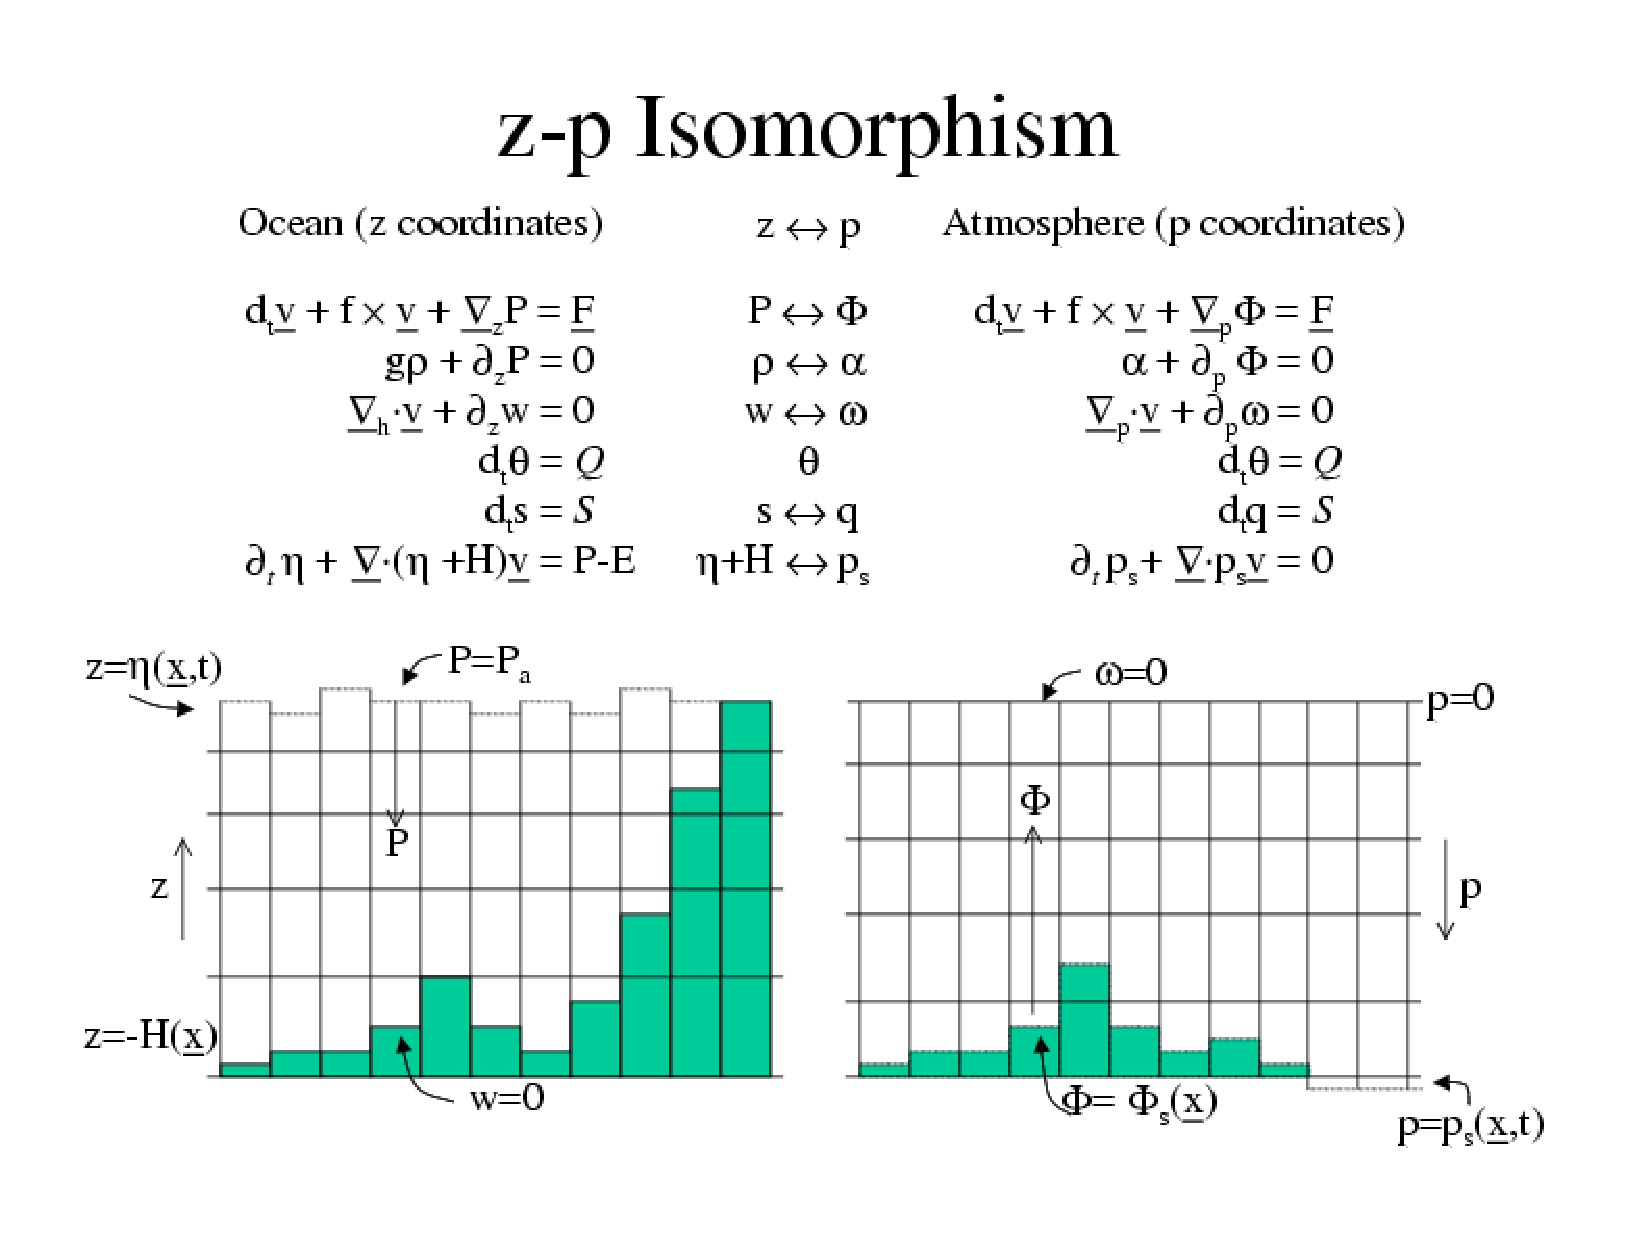
\includegraphics{part1/zandpcoord.eps}
  }
  \end{center}
\caption{Isomorphic equation sets used for atmosphere (right) and
ocean (left).}
\label{fig:isomorphic-equations}
\end{figure}

%%CNHend

The state of the fluid at any time is characterized by the distribution of
velocity $\vec{\mathbf{v}}$, active tracers $\theta $ and $S$, a
`geopotential' $\phi $ and density $\rho =\rho (\theta ,S,p)$ which may
depend on $\theta $, $S$, and $p$. The equations that govern the evolution
of these fields, obtained by applying the laws of classical mechanics and
thermodynamics to a Boussinesq, Navier-Stokes fluid are, written in terms of
a generic vertical coordinate, $r$, so that the appropriate
kinematic boundary conditions can be applied isomorphically
see figure \ref{fig:zandp-vert-coord}.

%%CNHbegin
\begin{figure}
  \begin{center}
   \rotatebox{-90}{
   \resizebox{!}{5.5in}{
   \includegraphics*[2.0in,3.0in][7.5in,10.5in]{part1/vertcoord.eps}
   }
   }
  \end{center}
\caption{Vertical coordinates and kinematic boundary conditions
for atmosphere (top) and ocean (bottom).}
\label{fig:zandp-vert-coord}
\end{figure}

%%CNHend

\begin{equation*}
\frac{D\vec{\mathbf{v}_{h}}}{Dt}+\left( 2\vec{\Omega}\times \vec{\mathbf{v}}
\right) _{h}+\mathbf{\nabla }_{h}\phi =\mathcal{F}_{\vec{\mathbf{v}_{h}}}
\text{ horizontal mtm} \label{eq:horizontal_mtm}
\end{equation*}

\begin{equation}
\frac{D\dot{r}}{Dt}+\widehat{k}\cdot \left( 2\vec{\Omega}\times \vec{\mathbf{
v}}\right) +\frac{\partial \phi }{\partial r}+b=\mathcal{F}_{\dot{r}}\text{
vertical mtm} \label{eq:vertical_mtm}
\end{equation}

\begin{equation}
\mathbf{\nabla }_{h}\cdot \vec{\mathbf{v}}_{h}+\frac{\partial \dot{r}}{
\partial r}=0\text{ continuity}  \label{eq:continuity}
\end{equation}

\begin{equation}
b=b(\theta ,S,r)\text{ equation of state} \label{eq:equation_of_state}
\end{equation}

\begin{equation}
\frac{D\theta }{Dt}=\mathcal{Q}_{\theta }\text{ potential temperature}
\label{eq:potential_temperature}
\end{equation}

\begin{equation}
\frac{DS}{Dt}=\mathcal{Q}_{S}\text{ humidity/salinity}
\label{eq:humidity_salt}
\end{equation}

Here:

\begin{equation*}
r\text{ is the vertical coordinate}
\end{equation*}

\begin{equation*}
\frac{D}{Dt}=\frac{\partial }{\partial t}+\vec{\mathbf{v}}\cdot \nabla \text{
is the total derivative}
\end{equation*}

\begin{equation*}
\mathbf{\nabla }=\mathbf{\nabla }_{h}+\widehat{k}\frac{\partial }{\partial r}
\text{ is the `grad' operator}
\end{equation*}
with $\mathbf{\nabla }_{h}$ operating in the horizontal and $\widehat{k}
\frac{\partial }{\partial r}$ operating in the vertical, where $\widehat{k}$
is a unit vector in the vertical

\begin{equation*}
t\text{ is time}
\end{equation*}

\begin{equation*}
\vec{\mathbf{v}}=(u,v,\dot{r})=(\vec{\mathbf{v}}_{h},\dot{r})\text{ is the
velocity}
\end{equation*}

\begin{equation*}
\phi \text{ is the `pressure'/`geopotential'}
\end{equation*}

\begin{equation*}
\vec{\Omega}\text{ is the Earth's rotation}
\end{equation*}

\begin{equation*}
b\text{ is the `buoyancy'}
\end{equation*}

\begin{equation*}
\theta \text{ is potential temperature}
\end{equation*}

\begin{equation*}
S\text{ is specific humidity in the atmosphere; salinity in the ocean}
\end{equation*}

\begin{equation*}
\mathcal{F}_{\vec{\mathbf{v}}}\text{ are forcing and dissipation of }\vec{
\mathbf{v}}
\end{equation*}

\begin{equation*}
\mathcal{Q}_{\theta }\mathcal{\ }\text{are forcing and dissipation of }\theta
\end{equation*}

\begin{equation*}
\mathcal{Q}_{S}\mathcal{\ }\text{are forcing and dissipation of }S
\end{equation*}

The $\mathcal{F}^{\prime }s$ and $\mathcal{Q}^{\prime }s$ are provided by
`physics' and forcing packages for atmosphere and ocean. These are described
in later chapters.

\subsection{Kinematic Boundary conditions}

\subsubsection{vertical}

at fixed and moving $r$ surfaces we set (see figure \ref{fig:zandp-vert-coord}):

\begin{equation}
\dot{r}=0 \text{\ at\ } r=R_{fixed}(x,y)\text{ (ocean bottom, top of the atmosphere)}
\label{eq:fixedbc}
\end{equation}

\begin{equation}
\dot{r}=\frac{Dr}{Dt} \text{\ at\ } r=R_{moving}\text{ \
(ocean surface,bottom of the atmosphere)}  \label{eq:movingbc}
\end{equation}

Here

\begin{equation*}
R_{moving}=R_{o}+\eta
\end{equation*}
where $R_{o}(x,y)$ is the `$r-$value' (height or pressure, depending on
whether we are in the atmosphere or ocean) of the `moving surface' in the
resting fluid and $\eta $ is the departure from $R_{o}(x,y)$ in the presence
of motion.

\subsubsection{horizontal}

\begin{equation}
\vec{\mathbf{v}}\cdot \vec{\mathbf{n}}=0  \label{eq:noflow}
\end{equation}
where $\vec{\mathbf{n}}$ is the normal to a solid boundary.

\subsection{Atmosphere}

In the atmosphere, (see figure \ref{fig:zandp-vert-coord}), we interpret:

\begin{equation}
r=p\text{ is the pressure}  \label{eq:atmos-r}
\end{equation}

\begin{equation}
\dot{r}=\frac{Dp}{Dt}=\omega \text{ is the vertical velocity in }p\text{
coordinates}  \label{eq:atmos-omega}
\end{equation}

\begin{equation}
\phi =g\,z\text{ is the geopotential height}  \label{eq:atmos-phi}
\end{equation}

\begin{equation}
b=\frac{\partial \Pi }{\partial p}\theta \text{ is the buoyancy}
\label{eq:atmos-b}
\end{equation}

\begin{equation}
\theta =T(\frac{p_{c}}{p})^{\kappa }\text{ is potential temperature}
\label{eq:atmos-theta}
\end{equation}

\begin{equation}
S=q,\text{ is the specific humidity}  \label{eq:atmos-s}
\end{equation}
where

\begin{equation*}
T\text{ is absolute temperature}
\end{equation*}
\begin{equation*}
p\text{ is the pressure}
\end{equation*}
\begin{eqnarray*}
&&z\text{ is the height of the pressure surface} \\
&&g\text{ is the acceleration due to gravity}
\end{eqnarray*}

In the above the ideal gas law, $p=\rho RT$, has been expressed in terms of
the Exner function $\Pi (p)$ given by (see Appendix Atmosphere) 
\begin{equation}
\Pi (p)=c_{p}(\frac{p}{p_{c}})^{\kappa }  \label{eq:exner}
\end{equation}
where $p_{c}$ is a reference pressure and $\kappa =R/c_{p}$ with $R$ the gas
constant and $c_{p}$ the specific heat of air at constant pressure.

At the top of the atmosphere (which is `fixed' in our $r$ coordinate):

\begin{equation*}
R_{fixed}=p_{top}=0
\end{equation*}
In a resting atmosphere the elevation of the mountains at the bottom is
given by 
\begin{equation*}
R_{moving}=R_{o}(x,y)=p_{o}(x,y)
\end{equation*}
i.e. the (hydrostatic) pressure at the top of the mountains in a resting
atmosphere.

The boundary conditions at top and bottom are given by:

\begin{eqnarray}
&&\omega =0~\text{at }r=R_{fixed} \text{ (top of the atmosphere)}
\label{eq:fixed-bc-atmos} \\
\omega &=&\frac{Dp_{s}}{Dt}\text{; at }r=R_{moving}\text{ (bottom of the
atmosphere)}  \label{eq:moving-bc-atmos}
\end{eqnarray}

Then the (hydrostatic form of) equations (\ref{eq:horizontal_mtm}-\ref{eq:humidity_salt}) 
yields a consistent set of atmospheric equations which, for convenience, are written out in $p$
coordinates in Appendix Atmosphere - see eqs(\ref{eq:atmos-prime}).

\subsection{Ocean}

In the ocean we interpret: 
\begin{eqnarray}
r &=&z\text{ is the height}  \label{eq:ocean-z} \\
\dot{r} &=&\frac{Dz}{Dt}=w\text{ is the vertical velocity}
\label{eq:ocean-w} \\
\phi &=&\frac{p}{\rho _{c}}\text{ is the pressure}  \label{eq:ocean-p} \\
b(\theta ,S,r) &=&\frac{g}{\rho _{c}}\left( \rho (\theta ,S,r)-\rho
_{c}\right) \text{ is the buoyancy}  \label{eq:ocean-b}
\end{eqnarray}
where $\rho _{c}$ is a fixed reference density of water and $g$ is the
acceleration due to gravity.\noindent

In the above

At the bottom of the ocean: $R_{fixed}(x,y)=-H(x,y)$.

The surface of the ocean is given by: $R_{moving}=\eta $

The position of the resting free surface of the ocean is given by $
R_{o}=Z_{o}=0$.

Boundary conditions are:

\begin{eqnarray}
w &=&0~\text{at }r=R_{fixed}\text{ (ocean bottom)}  \label{eq:fixed-bc-ocean}
\\
w &=&\frac{D\eta }{Dt}\text{ at }r=R_{moving}=\eta \text{ (ocean surface) 
\label{eq:moving-bc-ocean}}
\end{eqnarray}
where $\eta $ is the elevation of the free surface.

Then equations (\ref{eq:horizontal_mtm}-\ref{eq:humidity_salt}) yield a consistent set 
of oceanic equations
which, for convenience, are written out in $z$ coordinates in Appendix Ocean
- see eqs(\ref{eq:ocean-mom}) to (\ref{eq:ocean-salt}).

\subsection{Hydrostatic, Quasi-hydrostatic, Quasi-nonhydrostatic and
Non-hydrostatic forms}
\begin{rawhtml}
<!-- CMIREDIR:non_hydrostatic -->
\end{rawhtml}


Let us separate $\phi $ in to surface, hydrostatic and non-hydrostatic terms:

\begin{equation}
\phi (x,y,r)=\phi _{s}(x,y)+\phi _{hyd}(x,y,r)+\phi _{nh}(x,y,r)
\label{eq:phi-split}
\end{equation}
and write eq(\ref{eq:incompressible}) in the form:

\begin{equation}
\frac{\partial \vec{\mathbf{v}_{h}}}{\partial t}+\mathbf{\nabla }_{h}\phi
_{s}+\mathbf{\nabla }_{h}\phi _{hyd}+\epsilon _{nh}\mathbf{\nabla }_{h}\phi
_{nh}=\vec{\mathbf{G}}_{\vec{v}_{h}}  \label{eq:mom-h}
\end{equation}

\begin{equation}
\frac{\partial \phi _{hyd}}{\partial r}=-b  \label{eq:hydrostatic}
\end{equation}

\begin{equation}
\epsilon _{nh}\frac{\partial \dot{r}}{\partial t}+\frac{\partial \phi _{nh}}{
\partial r}=G_{\dot{r}}  \label{eq:mom-w}
\end{equation}
Here $\epsilon _{nh}$ is a non-hydrostatic parameter.

The $\left( \vec{\mathbf{G}}_{\vec{v}},G_{\dot{r}}\right) $ in eq(\ref
{eq:mom-h}) and (\ref{eq:mom-w}) represent advective, metric and Coriolis
terms in the momentum equations. In spherical coordinates they take the form
\footnote{
In the hydrostatic primitive equations (\textbf{HPE}) all underlined terms
in (\ref{eq:gu-speherical}), (\ref{eq:gv-spherical}) and (\ref
{eq:gw-spherical}) are omitted; the singly-underlined terms are included in
the quasi-hydrostatic model (\textbf{QH}). The fully non-hydrostatic model (
\textbf{NH}) includes all terms.} - see Marshall et al 1997a for a full
discussion:

\begin{equation}
\left. 
\begin{tabular}{l}
$G_{u}=-\vec{\mathbf{v}}.\nabla u$ \\ 
$-\left\{ \underline{\frac{u\dot{r}}{{r}}}-\frac{uv\tan \varphi}{{r}}\right\} $
\\ 
$-\left\{ -2\Omega v\sin \varphi+\underline{2\Omega \dot{r}\cos \varphi}\right\} $
\\ 
$+\mathcal{F}_{u}$
\end{tabular}
\ \right\} \left\{ 
\begin{tabular}{l}
\textit{advection} \\ 
\textit{metric} \\ 
\textit{Coriolis} \\ 
\textit{\ Forcing/Dissipation}
\end{tabular}
\ \right. \qquad  \label{eq:gu-speherical}
\end{equation}

\begin{equation}
\left. 
\begin{tabular}{l}
$G_{v}=-\vec{\mathbf{v}}.\nabla v$ \\ 
$-\left\{ \underline{\frac{v\dot{r}}{{r}}}-\frac{u^{2}\tan \varphi}{{r}}\right\} 
$ \\ 
$-\left\{ -2\Omega u\sin \varphi \right\} $ \\ 
$+\mathcal{F}_{v}$
\end{tabular}
\ \right\} \left\{ 
\begin{tabular}{l}
\textit{advection} \\ 
\textit{metric} \\ 
\textit{Coriolis} \\ 
\textit{\ Forcing/Dissipation}
\end{tabular}
\ \right. \qquad  \label{eq:gv-spherical}
\end{equation}
\qquad \qquad \qquad \qquad \qquad

\begin{equation}
\left. 
\begin{tabular}{l}
$G_{\dot{r}}=-\underline{\underline{\vec{\mathbf{v}}.\nabla \dot{r}}}$ \\ 
$+\left\{ \underline{\frac{u^{_{^{2}}}+v^{2}}{{r}}}\right\} $ \\ 
${+}\underline{{2\Omega u\cos \varphi}}$ \\ 
$\underline{\underline{\mathcal{F}_{\dot{r}}}}$
\end{tabular}
\ \right\} \left\{ 
\begin{tabular}{l}
\textit{advection} \\ 
\textit{metric} \\ 
\textit{Coriolis} \\ 
\textit{\ Forcing/Dissipation}
\end{tabular}
\ \right.  \label{eq:gw-spherical}
\end{equation}
\qquad \qquad \qquad \qquad \qquad

In the above `${r}$' is the distance from the center of the earth and `$\varphi$
' is latitude.

Grad and div operators in spherical coordinates are defined in appendix
OPERATORS.

%%CNHbegin
\begin{figure}
  \begin{center}
   \resizebox{5in}{!}{
   \includegraphics*[0.5in,0.5in][7.5in,10.5in]{part1/sphere.ps}
   }
  \end{center}
\caption{}
\label{fig:spherical-polar-coord}
\end{figure}

%%CNHend

\subsubsection{Shallow atmosphere approximation}

Most models are based on the `hydrostatic primitive equations' (HPE's) in
which the vertical momentum equation is reduced to a statement of
hydrostatic balance and the `traditional approximation' is made in which the
Coriolis force is treated approximately and the shallow atmosphere
approximation is made.\ The MITgcm need not make the `traditional
approximation'. To be able to support consistent non-hydrostatic forms the
shallow atmosphere approximation can be relaxed - when dividing through by $
r $ in, for example, (\ref{eq:gu-speherical}), we do not replace $r$ by $a$,
the radius of the earth.

\subsubsection{Hydrostatic and quasi-hydrostatic forms}
\label{sec:hydrostatic_and_quasi-hydrostatic_forms}

These are discussed at length in Marshall et al (1997a).

In the `hydrostatic primitive equations' (\textbf{HPE)} all the underlined
terms in Eqs. (\ref{eq:gu-speherical} $\rightarrow $\ \ref{eq:gw-spherical})
are neglected and `${r}$' is replaced by `$a$', the mean radius of the
earth. Once the pressure is found at one level - e.g. by inverting a 2-d
Elliptic equation for $\phi _{s}$ at $r=R_{moving}$ - the pressure can be
computed at all other levels by integration of the hydrostatic relation, eq(
\ref{eq:hydrostatic}).

In the `quasi-hydrostatic' equations (\textbf{QH)} strict balance between
gravity and vertical pressure gradients is not imposed. The $2\Omega u\cos
\varphi $ Coriolis term are not neglected and are balanced by a non-hydrostatic
contribution to the pressure field: only the terms underlined twice in Eqs. (
\ref{eq:gu-speherical}$\rightarrow $\ \ref{eq:gw-spherical}) are set to zero
and, simultaneously, the shallow atmosphere approximation is relaxed. In 
\textbf{QH}\ \textit{all} the metric terms are retained and the full
variation of the radial position of a particle monitored. The \textbf{QH}\
vertical momentum equation (\ref{eq:mom-w}) becomes:

\begin{equation*}
\frac{\partial \phi _{nh}}{\partial r}=2\Omega u\cos \varphi
\end{equation*}
making a small correction to the hydrostatic pressure.

\textbf{QH} has good energetic credentials - they are the same as for 
\textbf{HPE}. Importantly, however, it has the same angular momentum
principle as the full non-hydrostatic model (\textbf{NH)} - see Marshall
et.al., 1997a. As in \textbf{HPE }only a 2-d elliptic problem need be solved.

\subsubsection{Non-hydrostatic and quasi-nonhydrostatic forms}

The MIT model presently supports a full non-hydrostatic ocean isomorph, but
only a quasi-non-hydrostatic atmospheric isomorph.

\paragraph{Non-hydrostatic Ocean}

In the non-hydrostatic ocean model all terms in equations Eqs.(\ref
{eq:gu-speherical} $\rightarrow $\ \ref{eq:gw-spherical}) are retained. A
three dimensional elliptic equation must be solved subject to Neumann
boundary conditions (see below). It is important to note that use of the
full \textbf{NH} does not admit any new `fast' waves in to the system - the
incompressible condition eq(\ref{eq:continuity}) has already filtered out
acoustic modes. It does, however, ensure that the gravity waves are treated
accurately with an exact dispersion relation. The \textbf{NH} set has a
complete angular momentum principle and consistent energetics - see White
and Bromley, 1995; Marshall et.al.\ 1997a.

\paragraph{Quasi-nonhydrostatic Atmosphere}

In the non-hydrostatic version of our atmospheric model we approximate $\dot{
r}$ in the vertical momentum eqs(\ref{eq:mom-w}) and (\ref{eq:gv-spherical})
(but only here) by:

\begin{equation}
\dot{r}=\frac{Dp}{Dt}=\frac{1}{g}\frac{D\phi }{Dt}  \label{eq:quasi-nh-w}
\end{equation}
where $p_{hy}$ is the hydrostatic pressure.

\subsubsection{Summary of equation sets supported by model}

\paragraph{Atmosphere}

Hydrostatic, and quasi-hydrostatic and quasi non-hydrostatic forms of the
compressible non-Boussinesq equations in $p-$coordinates are supported.

\subparagraph{Hydrostatic and quasi-hydrostatic}

The hydrostatic set is written out in $p-$coordinates in appendix Atmosphere
- see eq(\ref{eq:atmos-prime}).

\subparagraph{Quasi-nonhydrostatic}

A quasi-nonhydrostatic form is also supported.

\paragraph{Ocean}

\subparagraph{Hydrostatic and quasi-hydrostatic}

Hydrostatic, and quasi-hydrostatic forms of the incompressible Boussinesq
equations in $z-$coordinates are supported.

\subparagraph{Non-hydrostatic}

Non-hydrostatic forms of the incompressible Boussinesq equations in $z-$
coordinates are supported - see eqs(\ref{eq:ocean-mom}) to (\ref
{eq:ocean-salt}).

\subsection{Solution strategy}

The method of solution employed in the \textbf{HPE}, \textbf{QH} and \textbf{
NH} models is summarized in Figure \ref{fig:solution-strategy}.
Under all dynamics, a 2-d elliptic equation is
first solved to find the surface pressure and the hydrostatic pressure at
any level computed from the weight of fluid above. Under \textbf{HPE} and 
\textbf{QH} dynamics, the horizontal momentum equations are then stepped
forward and $\dot{r}$ found from continuity. Under \textbf{NH} dynamics a
3-d elliptic equation must be solved for the non-hydrostatic pressure before
stepping forward the horizontal momentum equations; $\dot{r}$ is found by
stepping forward the vertical momentum equation.

%%CNHbegin
\begin{figure}
  \begin{center}
   \resizebox{5in}{!}{
   \includegraphics{s_overview/figs/solution_strategy.ps}
   }
  \end{center}
\caption{Basic solution strategy in MITgcm. {\bf HPE} and {\bf QH}
forms diagnose the vertical velocity, in {\bf NH} a prognostic
equation for the vertical velocity is integrated.}
\label{fig:solution-strategy}
\end{figure}

%%CNHend

There is no penalty in implementing \textbf{QH} over \textbf{HPE} except, of
course, some complication that goes with the inclusion of $\cos \varphi \ $
Coriolis terms and the relaxation of the shallow atmosphere approximation.
But this leads to negligible increase in computation. In \textbf{NH}, in
contrast, one additional elliptic equation - a three-dimensional one - must
be inverted for $p_{nh}$. However the `overhead' of the \textbf{NH} model is
essentially negligible in the hydrostatic limit (see detailed discussion in
Marshall et al, 1997) resulting in a non-hydrostatic algorithm that, in the
hydrostatic limit, is as computationally economic as the \textbf{HPEs}.

\subsection{Finding the pressure field}
\label{sec:finding_the_pressure_field}

Unlike the prognostic variables $u$, $v$, $w$, $\theta $ and $S$, the
pressure field must be obtained diagnostically. We proceed, as before, by
dividing the total (pressure/geo) potential in to three parts, a surface
part, $\phi _{s}(x,y)$, a hydrostatic part $\phi _{hyd}(x,y,r)$ and a
non-hydrostatic part $\phi _{nh}(x,y,r)$, as in (\ref{eq:phi-split}), and
writing the momentum equation as in (\ref{eq:mom-h}).

\subsubsection{Hydrostatic pressure}

Hydrostatic pressure is obtained by integrating (\ref{eq:hydrostatic})
vertically from $r=R_{o}$ where $\phi _{hyd}(r=R_{o})=0$, to yield:

\begin{equation*}
\int_{r}^{R_{o}}\frac{\partial \phi _{hyd}}{\partial r}dr=\left[ \phi _{hyd}
\right] _{r}^{R_{o}}=\int_{r}^{R_{o}}-bdr
\end{equation*}
and so

\begin{equation}
\phi _{hyd}(x,y,r)=\int_{r}^{R_{o}}bdr  \label{eq:hydro-phi}
\end{equation}

The model can be easily modified to accommodate a loading term (e.g
atmospheric pressure pushing down on the ocean's surface) by setting:

\begin{equation}
\phi _{hyd}(r=R_{o})=loading  \label{eq:loading}
\end{equation}

\subsubsection{Surface pressure}

The surface pressure equation can be obtained by integrating continuity,
(\ref{eq:continuity}), vertically from $r=R_{fixed}$ to $r=R_{moving}$

\begin{equation*}
\int_{R_{fixed}}^{R_{moving}}\left( \mathbf{\nabla }_{h}\cdot \vec{\mathbf{v}
}_{h}+\partial _{r}\dot{r}\right) dr=0
\end{equation*}

Thus:

\begin{equation*}
\frac{\partial \eta }{\partial t}+\vec{\mathbf{v}}.\nabla \eta
+\int_{R_{fixed}}^{R_{moving}}\mathbf{\nabla }_{h}\cdot \vec{\mathbf{v}}
_{h}dr=0
\end{equation*}
where $\eta =R_{moving}-R_{o}$ is the free-surface $r$-anomaly in units of $
r $. The above can be rearranged to yield, using Leibnitz's theorem:

\begin{equation}
\frac{\partial \eta }{\partial t}+\mathbf{\nabla }_{h}\cdot
\int_{R_{fixed}}^{R_{moving}}\vec{\mathbf{v}}_{h}dr=\text{source}
\label{eq:free-surface}
\end{equation}
where we have incorporated a source term.

Whether $\phi $ is pressure (ocean model, $p/\rho _{c}$) or geopotential
(atmospheric model), in (\ref{eq:mom-h}), the horizontal gradient term can
be written 
\begin{equation}
\mathbf{\nabla }_{h}\phi _{s}=\mathbf{\nabla }_{h}\left( b_{s}\eta \right)
\label{eq:phi-surf}
\end{equation}
where $b_{s}$ is the buoyancy at the surface.

In the hydrostatic limit ($\epsilon _{nh}=0$), equations (\ref{eq:mom-h}), (\ref
{eq:free-surface}) and (\ref{eq:phi-surf}) can be solved by inverting a 2-d
elliptic equation for $\phi _{s}$ as described in Chapter 2. Both `free
surface' and `rigid lid' approaches are available.

\subsubsection{Non-hydrostatic pressure}

Taking the horizontal divergence of (\ref{eq:mom-h}) and adding 
$\frac{\partial }{\partial r}$ of (\ref{eq:mom-w}), invoking the continuity equation
(\ref{eq:continuity}), we deduce that:

\begin{equation}
\nabla _{3}^{2}\phi _{nh}=\nabla .\vec{\mathbf{G}}_{\vec{v}}-\left( \mathbf{
\nabla }_{h}^{2}\phi _{s}+\mathbf{\nabla }^{2}\phi _{hyd}\right) =\nabla .
\vec{\mathbf{F}}  \label{eq:3d-invert}
\end{equation}

For a given rhs this 3-d elliptic equation must be inverted for $\phi _{nh}$
subject to appropriate choice of boundary conditions. This method is usually
called \textit{The Pressure Method} [Harlow and Welch, 1965; Williams, 1969;
Potter, 1976]. In the hydrostatic primitive equations case (\textbf{HPE}),
the 3-d problem does not need to be solved.

\paragraph{Boundary Conditions}

We apply the condition of no normal flow through all solid boundaries - the
coasts (in the ocean) and the bottom:

\begin{equation}
\vec{\mathbf{v}}.\widehat{n}=0  \label{nonormalflow}
\end{equation}
where $\widehat{n}$ is a vector of unit length normal to the boundary. The
kinematic condition (\ref{nonormalflow}) is also applied to the vertical
velocity at $r=R_{moving}$. No-slip $\left( v_{T}=0\right) \ $or slip $
\left( \partial v_{T}/\partial n=0\right) \ $conditions are employed on the
tangential component of velocity, $v_{T}$, at all solid boundaries,
depending on the form chosen for the dissipative terms in the momentum
equations - see below.

Eq.(\ref{nonormalflow}) implies, making use of (\ref{eq:mom-h}), that:

\begin{equation}
\widehat{n}.\nabla \phi _{nh}=\widehat{n}.\vec{\mathbf{F}}
\label{eq:inhom-neumann-nh}
\end{equation}
where

\begin{equation*}
\vec{\mathbf{F}}=\vec{\mathbf{G}}_{\vec{v}}-\left( \mathbf{\nabla }_{h}\phi
_{s}+\mathbf{\nabla }\phi _{hyd}\right) 
\end{equation*}
presenting inhomogeneous Neumann boundary conditions to the Elliptic problem
(\ref{eq:3d-invert}). As shown, for example, by Williams (1969), one can
exploit classical 3D potential theory and, by introducing an appropriately
chosen $\delta $-function sheet of `source-charge', replace the
inhomogeneous boundary condition on pressure by a homogeneous one. The
source term $rhs$ in (\ref{eq:3d-invert}) is the divergence of the vector $
\vec{\mathbf{F}}.$ By simultaneously setting $
\begin{array}{l}
\widehat{n}.\vec{\mathbf{F}}
\end{array}
=0$\ and $\widehat{n}.\nabla \phi _{nh}=0\ $on the boundary the following
self-consistent but simpler homogenized Elliptic problem is obtained:

\begin{equation*}
\nabla ^{2}\phi _{nh}=\nabla .\widetilde{\vec{\mathbf{F}}}\qquad
\end{equation*}
where $\widetilde{\vec{\mathbf{F}}}$ is a modified $\vec{\mathbf{F}}$ such
that $\widetilde{\vec{\mathbf{F}}}.\widehat{n}=0$. As is implied by (\ref
{eq:inhom-neumann-nh}) the modified boundary condition becomes:

\begin{equation}
\widehat{n}.\nabla \phi _{nh}=0  \label{eq:hom-neumann-nh}
\end{equation}

If the flow is `close' to hydrostatic balance then the 3-d inversion
converges rapidly because $\phi _{nh}\ $is then only a small correction to
the hydrostatic pressure field (see the discussion in Marshall et al, a,b).

The solution $\phi _{nh}\ $to (\ref{eq:3d-invert}) and (\ref{eq:inhom-neumann-nh})
does not vanish at $r=R_{moving}$, and so refines the pressure there.

\subsection{Forcing/dissipation}

\subsubsection{Forcing}

The forcing terms $\mathcal{F}$ on the rhs of the equations are provided by
`physics packages' and forcing packages. These are described later on.

\subsubsection{Dissipation}

\paragraph{Momentum}

Many forms of momentum dissipation are available in the model. Laplacian and
biharmonic frictions are commonly used:

\begin{equation}
D_{V}=A_{h}\nabla _{h}^{2}v+A_{v}\frac{\partial ^{2}v}{\partial z^{2}}
+A_{4}\nabla _{h}^{4}v  \label{eq:dissipation}
\end{equation}
where $A_{h}$ and $A_{v}\ $are (constant) horizontal and vertical viscosity
coefficients and $A_{4}\ $is the horizontal coefficient for biharmonic
friction. These coefficients are the same for all velocity components.

\paragraph{Tracers}

The mixing terms for the temperature and salinity equations have a similar
form to that of momentum except that the diffusion tensor can be
non-diagonal and have varying coefficients. $\qquad $
\begin{equation}
D_{T,S}=\nabla .[\underline{\underline{K}}\nabla (T,S)]+K_{4}\nabla
_{h}^{4}(T,S)  \label{eq:diffusion}
\end{equation}
where $\underline{\underline{K}}\ $is the diffusion tensor and the $K_{4}\ $
horizontal coefficient for biharmonic diffusion. In the simplest case where
the subgrid-scale fluxes of heat and salt are parameterized with constant
horizontal and vertical diffusion coefficients, $\underline{\underline{K}}$,
reduces to a diagonal matrix with constant coefficients:

\begin{equation}
\qquad \qquad \qquad \qquad K=\left( 
\begin{array}{ccc}
K_{h} & 0 & 0 \\ 
0 & K_{h} & 0 \\ 
0 & 0 & K_{v}
\end{array}
\right) \qquad \qquad \qquad  \label{eq:diagonal-diffusion-tensor}
\end{equation}
where $K_{h}\ $and $K_{v}\ $are the horizontal and vertical diffusion
coefficients. These coefficients are the same for all tracers (temperature,
salinity ... ).

\subsection{Vector invariant form}

For some purposes it is advantageous to write momentum advection in eq(\ref
{eq:horizontal_mtm}) and (\ref{eq:vertical_mtm}) in the (so-called) `vector invariant' form:

\begin{equation}
\frac{D\vec{\mathbf{v}}}{Dt}=\frac{\partial \vec{\mathbf{v}}}{\partial t}
+\left( \nabla \times \vec{\mathbf{v}}\right) \times \vec{\mathbf{v}}+\nabla 
\left[ \frac{1}{2}(\vec{\mathbf{v}}\cdot \vec{\mathbf{v}})\right]
\label{eq:vi-identity}
\end{equation}
This permits alternative numerical treatments of the non-linear terms based
on their representation as a vorticity flux. Because gradients of coordinate
vectors no longer appear on the rhs of (\ref{eq:vi-identity}), explicit
representation of the metric terms in (\ref{eq:gu-speherical}), (\ref
{eq:gv-spherical}) and (\ref{eq:gw-spherical}), can be avoided: information
about the geometry is contained in the areas and lengths of the volumes used
to discretize the model.

\subsection{Adjoint}

Tangent linear and adjoint counterparts of the forward model are described
in Chapter 5.

% $Header: /u/gcmpack/manual/s_overview/text/manual.tex,v 1.18 2004/03/23 15:29:39 afe Exp $
% $Name:  $

\section{Appendix ATMOSPHERE}

\subsection{Hydrostatic Primitive Equations for the Atmosphere in pressure
coordinates}

\label{sect-hpe-p}

The hydrostatic primitive equations (HPEs) in p-coordinates are: 
\begin{eqnarray}
\frac{D\vec{\mathbf{v}}_{h}}{Dt}+f\hat{\mathbf{k}}\times \vec{\mathbf{v}}
_{h}+\mathbf{\nabla }_{p}\phi &=&\vec{\mathbf{\mathcal{F}}}
\label{eq:atmos-mom} \\
\frac{\partial \phi }{\partial p}+\alpha &=&0  \label{eq-p-hydro-start} \\
\mathbf{\nabla }_{p}\cdot \vec{\mathbf{v}}_{h}+\frac{\partial \omega }{
\partial p} &=&0  \label{eq:atmos-cont} \\
p\alpha &=&RT  \label{eq:atmos-eos} \\
c_{v}\frac{DT}{Dt}+p\frac{D\alpha }{Dt} &=&\mathcal{Q}  \label{eq:atmos-heat}
\end{eqnarray}
where $\vec{\mathbf{v}}_{h}=(u,v,0)$ is the `horizontal' (on pressure
surfaces) component of velocity,$\frac{D}{Dt}=\vec{\mathbf{v}}_{h}\cdot 
\mathbf{\nabla }_{p}+\omega \frac{\partial }{\partial p}$ is the total
derivative, $f=2\Omega \sin \varphi$ is the Coriolis parameter, $\phi =gz$ is
the geopotential, $\alpha =1/\rho $ is the specific volume, $\omega =\frac{Dp
}{Dt}$ is the vertical velocity in the $p-$coordinate. Equation(\ref
{eq:atmos-heat}) is the first law of thermodynamics where internal energy $
e=c_{v}T$, $T$ is temperature, $Q$ is the rate of heating per unit mass and $
p\frac{D\alpha }{Dt}$ is the work done by the fluid in compressing.

It is convenient to cast the heat equation in terms of potential temperature 
$\theta $ so that it looks more like a generic conservation law.
Differentiating (\ref{eq:atmos-eos}) we get: 
\begin{equation*}
p\frac{D\alpha }{Dt}+\alpha \frac{Dp}{Dt}=R\frac{DT}{Dt}
\end{equation*}
which, when added to the heat equation (\ref{eq:atmos-heat}) and using $
c_{p}=c_{v}+R$, gives: 
\begin{equation}
c_{p}\frac{DT}{Dt}-\alpha \frac{Dp}{Dt}=\mathcal{Q}
\label{eq-p-heat-interim}
\end{equation}
Potential temperature is defined: 
\begin{equation}
\theta =T(\frac{p_{c}}{p})^{\kappa }  \label{eq:potential-temp}
\end{equation}
where $p_{c}$ is a reference pressure and $\kappa =R/c_{p}$. For convenience
we will make use of the Exner function $\Pi (p)$ which defined by: 
\begin{equation}
\Pi (p)=c_{p}(\frac{p}{p_{c}})^{\kappa }  \label{Exner}
\end{equation}
The following relations will be useful and are easily expressed in terms of
the Exner function: 
\begin{equation*}
c_{p}T=\Pi \theta \;\;;\;\;\frac{\partial \Pi }{\partial p}=\frac{\kappa \Pi 
}{p}\;\;;\;\;\alpha =\frac{\kappa \Pi \theta }{p}=\frac{\partial \ \Pi }{
\partial p}\theta \;\;;\;\;\frac{D\Pi }{Dt}=\frac{\partial \Pi }{\partial p}
\frac{Dp}{Dt}
\end{equation*}
where $b=\frac{\partial \ \Pi }{\partial p}\theta $ is the buoyancy.

The heat equation is obtained by noting that 
\begin{equation*}
c_{p}\frac{DT}{Dt}=\frac{D(\Pi \theta )}{Dt}=\Pi \frac{D\theta }{Dt}+\theta 
\frac{D\Pi }{Dt}=\Pi \frac{D\theta }{Dt}+\alpha \frac{Dp}{Dt}
\end{equation*}
and on substituting into (\ref{eq-p-heat-interim}) gives: 
\begin{equation}
\Pi \frac{D\theta }{Dt}=\mathcal{Q}
\label{eq:potential-temperature-equation}
\end{equation}
which is in conservative form.

For convenience in the model we prefer to step forward (\ref
{eq:potential-temperature-equation}) rather than (\ref{eq:atmos-heat}).

\subsubsection{Boundary conditions}

The upper and lower boundary conditions are : 
\begin{eqnarray}
\mbox{at the top:}\;\;p=0 &&\text{, }\omega =\frac{Dp}{Dt}=0 \\
\mbox{at the surface:}\;\;p=p_{s} &&\text{, }\phi =\phi _{topo}=g~Z_{topo}
\label{eq:boundary-condition-atmosphere}
\end{eqnarray}
In $p$-coordinates, the upper boundary acts like a solid boundary ($\omega
=0 $); in $z$-coordinates and the lower boundary is analogous to a free
surface ($\phi $ is imposed and $\omega \neq 0$).

\subsubsection{Splitting the geo-potential}

For the purposes of initialization and reducing round-off errors, the model
deals with perturbations from reference (or ``standard'') profiles. For
example, the hydrostatic geopotential associated with the resting atmosphere
is not dynamically relevant and can therefore be subtracted from the
equations. The equations written in terms of perturbations are obtained by
substituting the following definitions into the previous model equations: 
\begin{eqnarray}
\theta &=&\theta _{o}+\theta ^{\prime }  \label{eq:atmos-ref-prof-theta} \\
\alpha &=&\alpha _{o}+\alpha ^{\prime }  \label{eq:atmos-ref-prof-alpha} \\
\phi &=&\phi _{o}+\phi ^{\prime }  \label{eq:atmos-ref-prof-phi}
\end{eqnarray}
The reference state (indicated by subscript ``0'') corresponds to
horizontally homogeneous atmosphere at rest ($\theta _{o},\alpha _{o},\phi
_{o}$) with surface pressure $p_{o}(x,y)$ that satisfies $\phi
_{o}(p_{o})=g~Z_{topo}$, defined: 
\begin{eqnarray*}
\theta _{o}(p) &=&f^{n}(p) \\
\alpha _{o}(p) &=&\Pi _{p}\theta _{o} \\
\phi _{o}(p) &=&\phi _{topo}-\int_{p_{0}}^{p}\alpha _{o}dp
\end{eqnarray*}
%\begin{eqnarray*}
%\phi'_\alpha & = & \int^p_{p_o} (\alpha_o -\alpha) dp \\
%\phi'_s(x,y,t) & = & \int_{p_o}^{p_s} \alpha dp
%\end{eqnarray*}

The final form of the HPE's in p coordinates is then: 
\begin{eqnarray}
\frac{D\vec{\mathbf{v}}_{h}}{Dt}+f\hat{\mathbf{k}}\times \vec{\mathbf{v}}
_{h}+\mathbf{\nabla }_{p}\phi ^{\prime } &=&\vec{\mathbf{\mathcal{F}}} \label{eq:atmos-prime} \\
\frac{\partial \phi ^{\prime }}{\partial p}+\alpha ^{\prime } &=&0 \\
\mathbf{\nabla }_{p}\cdot \vec{\mathbf{v}}_{h}+\frac{\partial \omega }{
\partial p} &=&0 \\
\frac{\partial \Pi }{\partial p}\theta ^{\prime } &=&\alpha ^{\prime } \\
\frac{D\theta }{Dt} &=&\frac{\mathcal{Q}}{\Pi } 
\end{eqnarray}

% $Header: /u/gcmpack/manual/s_overview/text/manual.tex,v 1.18 2004/03/23 15:29:39 afe Exp $
% $Name:  $

\section{Appendix OCEAN}

\subsection{Equations of motion for the ocean}

We review here the method by which the standard (Boussinesq, incompressible)
HPE's for the ocean written in z-coordinates are obtained. The
non-Boussinesq equations for oceanic motion are: 
\begin{eqnarray}
\frac{D\vec{\mathbf{v}}_{h}}{Dt}+f\hat{\mathbf{k}}\times \vec{\mathbf{v}}
_{h}+\frac{1}{\rho }\mathbf{\nabla }_{z}p &=&\vec{\mathbf{\mathcal{F}}} \\
\epsilon _{nh}\frac{Dw}{Dt}+g+\frac{1}{\rho }\frac{\partial p}{\partial z}
&=&\epsilon _{nh}\mathcal{F}_{w} \\
\frac{1}{\rho }\frac{D\rho }{Dt}+\mathbf{\nabla }_{z}\cdot \vec{\mathbf{v}}
_{h}+\frac{\partial w}{\partial z} &=&0 \label{eq-zns-cont}\\
\rho &=&\rho (\theta ,S,p) \label{eq-zns-eos}\\
\frac{D\theta }{Dt} &=&\mathcal{Q}_{\theta } \label{eq-zns-heat}\\
\frac{DS}{Dt} &=&\mathcal{Q}_{s}  \label{eq-zns-salt}
\label{eq:non-boussinesq}
\end{eqnarray}
These equations permit acoustics modes, inertia-gravity waves,
non-hydrostatic motions, a geostrophic (Rossby) mode and a thermohaline
mode. As written, they cannot be integrated forward consistently - if we
step $\rho $ forward in (\ref{eq-zns-cont}), the answer will not be
consistent with that obtained by stepping (\ref{eq-zns-heat}) and (\ref
{eq-zns-salt}) and then using (\ref{eq-zns-eos}) to yield $\rho $. It is
therefore necessary to manipulate the system as follows. Differentiating the
EOS (equation of state) gives:

\begin{equation}
\frac{D\rho }{Dt}=\left. \frac{\partial \rho }{\partial \theta }\right|
_{S,p}\frac{D\theta }{Dt}+\left. \frac{\partial \rho }{\partial S}\right|
_{\theta ,p}\frac{DS}{Dt}+\left. \frac{\partial \rho }{\partial p}\right|
_{\theta ,S}\frac{Dp}{Dt}  \label{EOSexpansion}
\end{equation}

Note that $\frac{\partial \rho }{\partial p}=\frac{1}{c_{s}^{2}}$ is the
reciprocal of the sound speed ($c_{s}$) squared. Substituting into \ref{eq-zns-cont} gives: 
\begin{equation}
\frac{1}{\rho c_{s}^{2}}\frac{Dp}{Dt}+\mathbf{\nabla }_{z}\cdot \vec{\mathbf{
v}}+\partial _{z}w\approx 0  \label{eq-zns-pressure}
\end{equation}
where we have used an approximation sign to indicate that we have assumed
adiabatic motion, dropping the $\frac{D\theta }{Dt}$ and $\frac{DS}{Dt}$.
Replacing \ref{eq-zns-cont} with \ref{eq-zns-pressure} yields a system that
can be explicitly integrated forward: 
\begin{eqnarray}
\frac{D\vec{\mathbf{v}}_{h}}{Dt}+f\hat{\mathbf{k}}\times \vec{\mathbf{v}}
_{h}+\frac{1}{\rho }\mathbf{\nabla }_{z}p &=&\vec{\mathbf{\mathcal{F}}}
\label{eq-cns-hmom} \\
\epsilon _{nh}\frac{Dw}{Dt}+g+\frac{1}{\rho }\frac{\partial p}{\partial z}
&=&\epsilon _{nh}\mathcal{F}_{w}  \label{eq-cns-hydro} \\
\frac{1}{\rho c_{s}^{2}}\frac{Dp}{Dt}+\mathbf{\nabla }_{z}\cdot \vec{\mathbf{
v}}_{h}+\frac{\partial w}{\partial z} &=&0  \label{eq-cns-cont} \\
\rho &=&\rho (\theta ,S,p)  \label{eq-cns-eos} \\
\frac{D\theta }{Dt} &=&\mathcal{Q}_{\theta }  \label{eq-cns-heat} \\
\frac{DS}{Dt} &=&\mathcal{Q}_{s}  \label{eq-cns-salt}
\end{eqnarray}

\subsubsection{Compressible z-coordinate equations}

Here we linearize the acoustic modes by replacing $\rho $ with $\rho _{o}(z)$
wherever it appears in a product (ie. non-linear term) - this is the
`Boussinesq assumption'. The only term that then retains the full variation
in $\rho $ is the gravitational acceleration: 
\begin{eqnarray}
\frac{D\vec{\mathbf{v}}_{h}}{Dt}+f\hat{\mathbf{k}}\times \vec{\mathbf{v}}
_{h}+\frac{1}{\rho _{o}}\mathbf{\nabla }_{z}p &=&\vec{\mathbf{\mathcal{F}}}
\label{eq-zcb-hmom} \\
\epsilon _{nh}\frac{Dw}{Dt}+\frac{g\rho }{\rho _{o}}+\frac{1}{\rho _{o}}
\frac{\partial p}{\partial z} &=&\epsilon _{nh}\mathcal{F}_{w}
\label{eq-zcb-hydro} \\
\frac{1}{\rho _{o}c_{s}^{2}}\frac{Dp}{Dt}+\mathbf{\nabla }_{z}\cdot \vec{
\mathbf{v}}_{h}+\frac{\partial w}{\partial z} &=&0  \label{eq-zcb-cont} \\
\rho &=&\rho (\theta ,S,p)  \label{eq-zcb-eos} \\
\frac{D\theta }{Dt} &=&\mathcal{Q}_{\theta }  \label{eq-zcb-heat} \\
\frac{DS}{Dt} &=&\mathcal{Q}_{s}  \label{eq-zcb-salt}
\end{eqnarray}
These equations still retain acoustic modes. But, because the
``compressible'' terms are linearized, the pressure equation \ref
{eq-zcb-cont} can be integrated implicitly with ease (the time-dependent
term appears as a Helmholtz term in the non-hydrostatic pressure equation).
These are the \emph{truly} compressible Boussinesq equations. Note that the
EOS must have the same pressure dependency as the linearized pressure term,
ie. $\left. \frac{\partial \rho }{\partial p}\right| _{\theta ,S}=\frac{1}{
c_{s}^{2}}$, for consistency.

\subsubsection{`Anelastic' z-coordinate equations}

The anelastic approximation filters the acoustic mode by removing the
time-dependency in the continuity (now pressure-) equation (\ref{eq-zcb-cont}
). This could be done simply by noting that $\frac{Dp}{Dt}\approx -g\rho _{o}
\frac{Dz}{Dt}=-g\rho _{o}w$, but this leads to an inconsistency between
continuity and EOS. A better solution is to change the dependency on
pressure in the EOS by splitting the pressure into a reference function of
height and a perturbation: 
\begin{equation*}
\rho =\rho (\theta ,S,p_{o}(z)+\epsilon _{s}p^{\prime })
\end{equation*}
Remembering that the term $\frac{Dp}{Dt}$ in continuity comes from
differentiating the EOS, the continuity equation then becomes: 
\begin{equation*}
\frac{1}{\rho _{o}c_{s}^{2}}\left( \frac{Dp_{o}}{Dt}+\epsilon _{s}\frac{
Dp^{\prime }}{Dt}\right) +\mathbf{\nabla }_{z}\cdot \vec{\mathbf{v}}_{h}+
\frac{\partial w}{\partial z}=0
\end{equation*}
If the time- and space-scales of the motions of interest are longer than
those of acoustic modes, then $\frac{Dp^{\prime }}{Dt}<<(\frac{Dp_{o}}{Dt},
\mathbf{\nabla }\cdot \vec{\mathbf{v}}_{h})$ in the continuity equations and 
$\left. \frac{\partial \rho }{\partial p}\right| _{\theta ,S}\frac{
Dp^{\prime }}{Dt}<<\left. \frac{\partial \rho }{\partial p}\right| _{\theta
,S}\frac{Dp_{o}}{Dt}$ in the EOS (\ref{EOSexpansion}). Thus we set $\epsilon
_{s}=0$, removing the dependency on $p^{\prime }$ in the continuity equation
and EOS. Expanding $\frac{Dp_{o}(z)}{Dt}=-g\rho _{o}w$ then leads to the
anelastic continuity equation: 
\begin{equation}
\mathbf{\nabla }_{z}\cdot \vec{\mathbf{v}}_{h}+\frac{\partial w}{\partial z}-
\frac{g}{c_{s}^{2}}w=0  \label{eq-za-cont1}
\end{equation}
A slightly different route leads to the quasi-Boussinesq continuity equation
where we use the scaling $\frac{\partial \rho ^{\prime }}{\partial t}+
\mathbf{\nabla }_{3}\cdot \rho ^{\prime }\vec{\mathbf{v}}<<\mathbf{\nabla }
_{3}\cdot \rho _{o}\vec{\mathbf{v}}$ yielding: 
\begin{equation}
\mathbf{\nabla }_{z}\cdot \vec{\mathbf{v}}_{h}+\frac{1}{\rho _{o}}\frac{
\partial \left( \rho _{o}w\right) }{\partial z}=0  \label{eq-za-cont2}
\end{equation}
Equations \ref{eq-za-cont1} and \ref{eq-za-cont2} are in fact the same
equation if: 
\begin{equation}
\frac{1}{\rho _{o}}\frac{\partial \rho _{o}}{\partial z}=\frac{-g}{c_{s}^{2}}
\end{equation}
Again, note that if $\rho _{o}$ is evaluated from prescribed $\theta _{o}$
and $S_{o}$ profiles, then the EOS dependency on $p_{o}$ and the term $\frac{
g}{c_{s}^{2}}$ in continuity should be referred to those same profiles. The
full set of `quasi-Boussinesq' or `anelastic' equations for the ocean are
then: 
\begin{eqnarray}
\frac{D\vec{\mathbf{v}}_{h}}{Dt}+f\hat{\mathbf{k}}\times \vec{\mathbf{v}}
_{h}+\frac{1}{\rho _{o}}\mathbf{\nabla }_{z}p &=&\vec{\mathbf{\mathcal{F}}}
\label{eq-zab-hmom} \\
\epsilon _{nh}\frac{Dw}{Dt}+\frac{g\rho }{\rho _{o}}+\frac{1}{\rho _{o}}
\frac{\partial p}{\partial z} &=&\epsilon _{nh}\mathcal{F}_{w}
\label{eq-zab-hydro} \\
\mathbf{\nabla }_{z}\cdot \vec{\mathbf{v}}_{h}+\frac{1}{\rho _{o}}\frac{
\partial \left( \rho _{o}w\right) }{\partial z} &=&0  \label{eq-zab-cont} \\
\rho &=&\rho (\theta ,S,p_{o}(z))  \label{eq-zab-eos} \\
\frac{D\theta }{Dt} &=&\mathcal{Q}_{\theta }  \label{eq-zab-heat} \\
\frac{DS}{Dt} &=&\mathcal{Q}_{s}  \label{eq-zab-salt}
\end{eqnarray}

\subsubsection{Incompressible z-coordinate equations}

Here, the objective is to drop the depth dependence of $\rho _{o}$ and so,
technically, to also remove the dependence of $\rho $ on $p_{o}$. This would
yield the ``truly'' incompressible Boussinesq equations: 
\begin{eqnarray}
\frac{D\vec{\mathbf{v}}_{h}}{Dt}+f\hat{\mathbf{k}}\times \vec{\mathbf{v}}
_{h}+\frac{1}{\rho _{c}}\mathbf{\nabla }_{z}p &=&\vec{\mathbf{\mathcal{F}}}
\label{eq-ztb-hmom} \\
\epsilon _{nh}\frac{Dw}{Dt}+\frac{g\rho }{\rho _{c}}+\frac{1}{\rho _{c}}
\frac{\partial p}{\partial z} &=&\epsilon _{nh}\mathcal{F}_{w}
\label{eq-ztb-hydro} \\
\mathbf{\nabla }_{z}\cdot \vec{\mathbf{v}}_{h}+\frac{\partial w}{\partial z}
&=&0  \label{eq-ztb-cont} \\
\rho &=&\rho (\theta ,S)  \label{eq-ztb-eos} \\
\frac{D\theta }{Dt} &=&\mathcal{Q}_{\theta }  \label{eq-ztb-heat} \\
\frac{DS}{Dt} &=&\mathcal{Q}_{s}  \label{eq-ztb-salt}
\end{eqnarray}
where $\rho _{c}$ is a constant reference density of water.

\subsubsection{Compressible non-divergent equations}

The above ``incompressible'' equations are incompressible in both the flow
and the density. In many oceanic applications, however, it is important to
retain compressibility effects in the density. To do this we must split the
density thus: 
\begin{equation*}
\rho =\rho _{o}+\rho ^{\prime }
\end{equation*}
We then assert that variations with depth of $\rho _{o}$ are unimportant
while the compressible effects in $\rho ^{\prime }$ are: 
\begin{equation*}
\rho _{o}=\rho _{c}
\end{equation*}
\begin{equation*}
\rho ^{\prime }=\rho (\theta ,S,p_{o}(z))-\rho _{o}
\end{equation*}
This then yields what we can call the semi-compressible Boussinesq
equations: 
\begin{eqnarray}
\frac{D\vec{\mathbf{v}}_{h}}{Dt}+f\hat{\mathbf{k}}\times \vec{\mathbf{v}}
_{h}+\frac{1}{\rho _{c}}\mathbf{\nabla }_{z}p^{\prime } &=&\vec{\mathbf{
\mathcal{F}}}  \label{eq:ocean-mom} \\
\epsilon _{nh}\frac{Dw}{Dt}+\frac{g\rho ^{\prime }}{\rho _{c}}+\frac{1}{\rho
_{c}}\frac{\partial p^{\prime }}{\partial z} &=&\epsilon _{nh}\mathcal{F}_{w}
\label{eq:ocean-wmom} \\
\mathbf{\nabla }_{z}\cdot \vec{\mathbf{v}}_{h}+\frac{\partial w}{\partial z}
&=&0  \label{eq:ocean-cont} \\
\rho ^{\prime } &=&\rho (\theta ,S,p_{o}(z))-\rho _{c}  \label{eq:ocean-eos}
\\
\frac{D\theta }{Dt} &=&\mathcal{Q}_{\theta }  \label{eq:ocean-theta} \\
\frac{DS}{Dt} &=&\mathcal{Q}_{s}  \label{eq:ocean-salt}
\end{eqnarray}
Note that the hydrostatic pressure of the resting fluid, including that
associated with $\rho _{c}$, is subtracted out since it has no effect on the
dynamics.

Though necessary, the assumptions that go into these equations are messy
since we essentially assume a different EOS for the reference density and
the perturbation density. Nevertheless, it is the hydrostatic ($\epsilon
_{nh}=0$ form of these equations that are used throughout the ocean modeling
community and referred to as the primitive equations (HPE).

% $Header: /u/gcmpack/manual/s_overview/text/manual.tex,v 1.18 2004/03/23 15:29:39 afe Exp $
% $Name:  $

\section{Appendix:OPERATORS}

\subsection{Coordinate systems}

\subsubsection{Spherical coordinates}

In spherical coordinates, the velocity components in the zonal, meridional
and vertical direction respectively, are given by (see Fig.2) :

\begin{equation*}
u=r\cos \varphi \frac{D\lambda }{Dt}
\end{equation*}

\begin{equation*}
v=r\frac{D\varphi }{Dt}\qquad
\end{equation*}
$\qquad \qquad \qquad \qquad $

\begin{equation*}
\dot{r}=\frac{Dr}{Dt}
\end{equation*}

Here $\varphi $ is the latitude, $\lambda $ the longitude, $r$ the radial
distance of the particle from the center of the earth, $\Omega $ is the
angular speed of rotation of the Earth and $D/Dt$ is the total derivative.

The `grad' ($\nabla $) and `div' ($\nabla $.) operators are defined by, in
spherical coordinates:

\begin{equation*}
\nabla \equiv \left( \frac{1}{r\cos \varphi }\frac{\partial }{\partial \lambda }
,\frac{1}{r}\frac{\partial }{\partial \varphi },\frac{\partial }{\partial r}
\right)
\end{equation*}

\begin{equation*}
\nabla .v\equiv \frac{1}{r\cos \varphi }\left\{ \frac{\partial u}{\partial
\lambda }+\frac{\partial }{\partial \varphi }\left( v\cos \varphi \right) \right\}
+\frac{1}{r^{2}}\frac{\partial \left( r^{2}\dot{r}\right) }{\partial r}
\end{equation*}

%tci%\end{document}
